\documentclass[12pt]{article}
\usepackage{amsmath, amsthm, amssymb}
\usepackage{hyperref}
\usepackage{verbatim}
\usepackage[top=1.0in, bottom=1.0in, left=1.0in, right=1.0in]{geometry}

\pagestyle{plain}

\usepackage{tkz-graph}
\usetikzlibrary{arrows}
\usetikzlibrary{shapes}
\usepackage[position=bottom]{subfig}

\usepackage{longtable}
\usepackage{array}

\usepackage{sectsty}
\allsectionsfont{\sffamily}

\setcounter{secnumdepth}{5}
\setcounter{tocdepth}{5}

\makeatletter
\newtheorem*{rep@theorem}{\rep@title}
\newcommand{\newreptheorem}[2]{
\newenvironment{rep#1}[1]{
 \def\rep@title{#2 \ref{##1}}
 \begin{rep@theorem}}
 {\end{rep@theorem}}}
\makeatother

\theoremstyle{plain}
\newtheorem{thm}{Theorem}[section]
\newreptheorem{thm}{Theorem}
\newtheorem{prop}[thm]{Proposition}
\newreptheorem{prop}{Proposition}
\newtheorem{lem}[thm]{Lemma}
\newreptheorem{lem}{Lemma}
\newtheorem{conjecture}[thm]{Conjecture}
\newreptheorem{conjecture}{Conjecture}
\newtheorem{cor}[thm]{Corollary}
\newreptheorem{cor}{Corollary}
\newtheorem{prob}[thm]{Problem}
\newtheorem{observation}{Observation}
\newtheorem*{mainconj}{Main Conjecture}
\newtheorem*{mainthm}{Main Theorem}

\theoremstyle{definition}
\newtheorem{defn}{Definition}
\theoremstyle{remark}
\newtheorem*{remark}{Remark}
\newtheorem*{problem}{Problem}
\newtheorem{example}{Example}
\newtheorem*{question}{Question}


\newcommand{\fancy}[1]{\mathcal{#1}}
\newcommand{\C}[1]{\fancy{C}_{#1}}
\newcommand{\IN}{\mathbb{N}}
\newcommand{\IR}{\mathbb{R}}
\newcommand{\G}{\fancy{G}}
\newcommand{\CC}{\fancy{C}}
\newcommand{\D}{\fancy{D}}

\newcommand{\inj}{\hookrightarrow}
\newcommand{\surj}{\twoheadrightarrow}

\newcommand{\set}[1]{\left\{ #1 \right\}}
\newcommand{\setb}[3]{\left\{ #1 \in #2 \mid #3 \right\}}
\newcommand{\setbs}[2]{\left\{ #1 \mid #2 \right\}}
\newcommand{\card}[1]{\left|#1\right|}
\newcommand{\size}[1]{\left\Vert#1\right\Vert}
\newcommand{\ceil}[1]{\left\lceil#1\right\rceil}
\newcommand{\floor}[1]{\left\lfloor#1\right\rfloor}
\newcommand{\func}[3]{#1\colon #2 \rightarrow #3}
\newcommand{\funcinj}[3]{#1\colon #2 \inj #3}
\newcommand{\funcsurj}[3]{#1\colon #2 \surj #3}
\newcommand{\irange}[1]{\left[#1\right]}
\newcommand{\join}[2]{#1 \mbox{\hspace{2 pt}$\ast$\hspace{2 pt}} #2}
\newcommand{\djunion}[2]{#1 \mbox{\hspace{2 pt}$+$\hspace{2 pt}} #2}
\newcommand{\parens}[1]{\left( #1 \right)}
\newcommand{\brackets}[1]{\left[ #1 \right]}
\newcommand{\nint}[1]{\widetilde{N}\left(#1\right)}
\newcommand{\DefinedAs}{\mathrel{\mathop:}=}
\newcommand{\pot}{\operatorname{pot}}

\def\adj{\leftrightarrow}
\def\nonadj{\not\!\leftrightarrow}

\def\D{\fancy{D}}
\def\C{\fancy{C}}
\def\Q{\fancy{Q}}
\def\Z{\fancy{Z}}

\newcommand{\case}[2]{{\bf Case #1.}~{\it #2}~~}
\newcommand{\claim}[2]{{\bf Claim #1.}~{\it #2}~~}

\newcommand{\wild}{\raisebox{0.75\depth}{$\bigstar$}}

\begin{document}
\title{fixable proofs}
\maketitle

\section{Proofs}
\begin{figure}
	\centering
	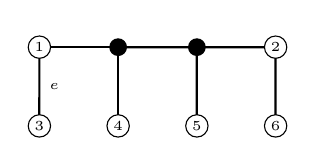
\begin{tikzpicture}[scale = 10]
	\tikzstyle{VertexStyle} = []
	\tikzstyle{EdgeStyle} = []
	\tikzstyle{labeledStyle}=[shape = circle, minimum size = 6pt, inner sep = 1.2pt, draw]
	\tikzstyle{unlabeledStyle}=[shape = circle, minimum size = 6pt, inner sep = 1.2pt, draw, fill]
	\Vertex[style = labeledStyle, x = 0.55, y = 0.75, L = \tiny {$1$}]{v0}
	\Vertex[style = unlabeledStyle, x = 0.65, y = 0.75, L = \tiny {}]{v1}
	\Vertex[style = unlabeledStyle, x = 0.75, y = 0.75, L = \tiny {}]{v2}
	\Vertex[style = labeledStyle, x = 0.85, y = 0.75, L = \tiny {$2$}]{v3}
	\Vertex[style = labeledStyle, x = 0.55, y = 0.65, L = \tiny {$3$}]{v4}
	\Vertex[style = labeledStyle, x = 0.65, y = 0.65, L = \tiny {$4$}]{v5}
	\Vertex[style = labeledStyle, x = 0.75, y = 0.65, L = \tiny {$5$}]{v6}
	\Vertex[style = labeledStyle, x = 0.85, y = 0.65, L = \tiny {$6$}]{v7}
	\Edge[label = \tiny {}, labelstyle={auto=right, fill=none}](v1)(v0)
	\Edge[label = \tiny {}, labelstyle={auto=right, fill=none}](v1)(v2)
	\Edge[label = \tiny {}, labelstyle={auto=right, fill=none}](v1)(v5)
	\Edge[label = \tiny {}, labelstyle={auto=right, fill=none}](v3)(v2)
	\Edge[label = \tiny {}, labelstyle={auto=right, fill=none}](v3)(v7)
	\Edge[label = \tiny {$e$}, labelstyle={auto=right, fill=none}](v4)(v0)
	\Edge[label = \tiny {}, labelstyle={auto=right, fill=none}](v6)(v2)
	\end{tikzpicture}
	
	\caption{Solid vertices have lists of size 3 and the labeled vertices have lists of size 2.}\label{fig:b860e768-7266-42fa-9d05-3beefaf3786e}
\end{figure}
\begin{lem}
	The graph in Figure \ref{fig:b860e768-7266-42fa-9d05-3beefaf3786e} is reducible.
\end{lem}
\begin{proof}Let $X = \{0,1\}$, $Y = \{0,2\}$ and $Z = \{1,2\}$. Then with the vertex ordering in Figure \ref{fig:b860e768-7266-42fa-9d05-3beefaf3786e}, a string such as ZXYXXX, 
	represents a possible list assignment on $V(H)$ arising from a $3$-edge-coloring of $G-E(H)$.
	By an $X$-Kempe change, we mean flipping colors $0$ and $1$ on a two-colored path in $G-E(H)$.  We call such a path an $X$-path. 
	Any endpoint of an $X$-path in $H$ must end at a $Y$ or $Z$ vertex.  The meanings of $Y$-Kempe change, $Z$-Kempe change, $Y$-path and $Z$-path are analogous.
	Note that if there are an odd number of $Y$'s and $Z$'s, then at least one $X$-Kempe change has only one endpoint in $H$.
	
	We need to handle all boards that are nearly colorable for edge $e$ up to permutations of $\{X,Y,Z\}$, so it will suffice to handle all boards of the form $\wild Z\wild \wild YZ$, $\wild \wild \wild YYZ$, $Y\wild \wild \wild YZ$, $X\wild \wild YZZ$, $Z\wild \wild YZZ$, $X\wild \wild ZYZ$, $Z\wild \wild XYZ$, $X\wild YZZZ$, $Y\wild YZZZ$, $YY\wild YZZ$, $YX\wild YZZ$, $XYZZZZ$, $YYZZZZ$, $YZZZZZ$, $ZZZZZZ$ or $ZZYZZZ$.
	
	\case{1}{$B$ is one of $\wild Z\wild \wild YZ$, $\wild Y\wild YZZ$, $\wild X\wild YZZ$, $\wild \wild ZYYZ$, $\wild \wild XYYZ$, $Y\wild Y\wild YZ$, $\wild ZYZZZ$, $X\wild ZZYZ$, $X\wild XZYZ$, $Y\wild YZZZ$, $Y\wild ZZYZ$, $Y\wild XXYZ$, $Z\wild ZXYZ$, $Z\wild XXYZ$, $XYZZZZ$, $XZYYZZ$, $XZXYZZ$, $YYZZZZ$, $ZZZZZZ$, $ZZZYZZ$ or $ZZYYZZ$.}
	In all these cases, $H$ is immediately colorable from the lists.
	
	\case{2}{$B$ is one of $XYY\wild YZ$, $XXYXYZ$, $XXYZYZ$, $XZZYZZ$, $XYYZZZ$, $YZZYZZ$, $YYXZYZ$, $YZZZZZ$, $ZYYZZZ$, $ZYZZYZ$, $ZYYYYZ$, $ZYXZYZ$, $ZXYZYZ$, $ZXZZYZ$, $ZXYZZZ$, $ZXYYYZ$ or $ZYZZZZ$.}
	
	
	For YZZZZZ, if the Y-path starting at the third vertex doesn't end in $H$ or ends at the fourth, fifth or sixth vertex of $H$, then doing a Y-Kempe change there yields XZYZZZ, XZYYZZ, XZYZYZ and XYZYYZ respectively, which are handled by Case 1.
	If the Y-path starting at the fifth vertex doesn't end in $H$ or ends at the fourth or sixth vertex of $H$, then doing a Y-Kempe change there yields XZZZYZ, XZZYYZ and XYYYZZ respectively, which are handled by Case 1.
	If the Y-path starting at the second vertex doesn't end in $H$ then doing a Y-Kempe change there yields XYZZZZ, which is handled by Case 1.
	Since we already handled the permutation of all resulting boards by (2 1 4 3 6 5), we have also handled ZYZZZZ.
	
	
	For XYYZZZ, if the X-path starting at the third vertex doesn't end in $H$ or ends at the fourth or sixth vertex of $H$, then doing an X-Kempe change there yields XYZZZZ, XYZYZZ and XZYYYZ respectively, which are handled by Case 1.
	If the X-path starting at the fourth vertex doesn't end in $H$ or ends at the sixth vertex of $H$, then doing an X-Kempe change there yields XYYYZZ and XZZZYZ respectively, which are handled by Case 1.
	If the X-path starting at the second vertex doesn't end in $H$ then doing an X-Kempe change there yields XZYZZZ, which is handled by Case 1.
	If the X-path starting at the sixth vertex doesn't end in $H$ then doing an X-Kempe change there yields XZZYYZ, which is handled by Case 1.
	Since we already handled the permutation of all resulting boards by (2 1 6 3 4 5), we have also handled ZXYYYZ.
	
	
	For XZZYZZ, if the X-path starting at the third vertex doesn't end in $H$ or ends at the second, fourth, fifth or sixth vertex of $H$, then doing an X-Kempe change there yields XZYYZZ, XYYYZZ, XZYZZZ, XZYYYZ and XYZZYZ respectively, which are handled by Case 1.
	If the X-path starting at the fifth vertex doesn't end in $H$ or ends at the fourth vertex of $H$, then doing an X-Kempe change there yields XZZYYZ and XZZZYZ respectively, which are handled by Case 1.
	If the X-path starting at the second vertex doesn't end in $H$ then doing an X-Kempe change there yields XYZYZZ, which is handled by Case 1.
	Since we already handled the permutation of all resulting boards by (1 2 3 6 5 4), (2 1 6 3 4 5) and (2 1 6 5 4 3), we have also handled XYYYYZ, ZXYZZZ and ZXZZYZ.
	
	
	For XYYZYZ, if the X-path starting at the third vertex doesn't end in $H$ or ends at the second, fourth, fifth or sixth vertex of $H$, then doing an X-Kempe change there yields XYZZYZ, XZZZYZ, XYZYYZ, XYZZZZ and XZYYZZ respectively, which are handled by Case 1.
	If the X-path starting at the second vertex doesn't end in $H$ then doing an X-Kempe change there yields XZYZYZ, which is handled by Case 1.
	If the X-path starting at the fifth vertex ends at the fourth or sixth vertex of $H$, then doing an X-Kempe change there yields XYYYZZ and XZZYYZ respectively, which are handled by Case 1.
	Since we already handled the permutation of all resulting boards by (2 1 6 3 4 5), we have also handled ZXYZYZ.
	
	
	For XXYZYZ, if the X-path starting at the fourth vertex ends at the fifth or sixth vertex of $H$, then doing an X-Kempe change there yields XXYYZZ and YYZZZZ respectively, which are handled by Case 1.
	If the X-path starting at the fifth vertex ends at the sixth vertex of $H$, then doing an X-Kempe change there yields XXZYYZ, which is handled by Case 1.
	
	For YYXZYZ, if the X-path starting at the fourth vertex doesn't end in $H$ or ends at the second, fifth or sixth vertex of $H$, then doing an X-Kempe change there yields YYXYYZ, YZXYYZ, YYXYZZ and ZZYZZZ respectively, which are handled by Case 1.
	If the X-path starting at the second vertex doesn't end in $H$ or ends at the fifth or sixth vertex of $H$, then doing an X-Kempe change there yields YZXZYZ, XZYZZZ and ZYXYZZ respectively, which are handled by Case 1.
	If the X-path starting at the fifth vertex ends at the sixth vertex of $H$, then doing an X-Kempe change there yields ZZXYYZ, which is handled by Case 1.
	Since we already handled the permutation of all resulting boards by (1 4 3 2 6 5), (2 1 6 5 4 3) and (2 5 6 1 3 4), we have also handled ZYXZYZ, XXYXYZ and XYYXYZ.
	
	
	For ZYYYYZ, if the X-path starting at the third vertex ends at the second, fifth or sixth vertex of $H$, then doing an X-Kempe change there yields ZZZYYZ, ZYZYZZ and YZYZZZ respectively, which are handled by Case 1.
	If the X-path starting at the fifth vertex ends at the second or sixth vertex of $H$, then doing an X-Kempe change there yields ZZYYZZ and YZZZYZ respectively, which are handled by Case 1.
	If the X-path starting at the second vertex ends at the sixth vertex of $H$, then doing an X-Kempe change there yields YYZZZZ, which is handled by Case 1.
	Since we already handled the permutation of all resulting boards by (1 2 3 6 5 4), (2 1 4 3 6 5) and (2 1 4 5 6 3), we have also handled YZZYZZ, ZYZZYZ and ZYYZZZ.
	
	
	\case{3}{$B$ is one of $XYXXYZ$, $XYZXYZ$, $XXXXYZ$, $XXZXYZ$, $XXYYYZ$, $XXYZZZ$, $YZXYZZ$, $YXXZYZ$, $YYZXYZ$, $ZXXZYZ$, $ZYYXYZ$, $ZXYXYZ$ or $ZZXYZZ$.}
	
	Since XXYZZZ has an odd number of X's and Y's, there is a Z-path with exactly one end in $H$.
	If this is the first, second or third vertex of $H$, then doing a Z-Kempe change there yields YXYZZZ, XYYZZZ and YYYZZZ respectively, which are handled by Cases 1 and 2.
	Since we already handled the permutation of all resulting boards by (1 2 6 3 4 5), (3 6 4 1 2 5) and (3 6 5 1 2 4), we have also handled XXYYYZ, YYZXYZ and XXZXYZ.
	
	
	For YXXZYZ, if the Z-path starting at the second vertex ends at the third or fifth vertex of $H$, then doing a Z-Kempe change there yields YYYZYZ and XXYZYZ respectively, which are handled by Cases 1 and 2.
	If the Z-path starting at the third vertex ends at the fifth vertex of $H$, then doing a Z-Kempe change there yields XYXZYZ, which is handled by Case 1.
	Since we already handled the permutation of all resulting boards by (1 2 4 3 6 5) and (1 3 6 2 4 5), we have also handled ZXYXYZ and XYZXYZ.
	
	
	For ZYYXYZ, if the Z-path starting at the third vertex ends at the fourth or fifth vertex of $H$, then doing a Z-Kempe change there yields ZYXYYZ and ZXYYYZ respectively, which are handled by Cases 1 and 2.
	If the Z-path starting at the fourth vertex ends at the fifth vertex of $H$, then doing a Z-Kempe change there yields ZXXXYZ, which is handled by Case 1.
	Since we already handled the permutation of all resulting boards by (1 2 5 3 6 4), (2 1 3 6 4 5) and (2 1 4 5 6 3), we have also handled YZXYZZ, XYXXYZ and ZXXZYZ.
	
	
	For ZZXYZZ, if the Y-path starting at the third vertex doesn't end in $H$ or ends at the first, second or fifth vertex of $H$, then doing a Y-Kempe change there yields ZZZYZZ, XZZYZZ, ZXZYZZ and ZZZXYZ respectively, which are handled by Cases 1 and 2.
	If the Y-path starting at the first vertex doesn't end in $H$ then doing a Y-Kempe change there yields XZXYZZ, which is handled by Case 1.
	If the Y-path starting at the second vertex doesn't end in $H$ then doing a Y-Kempe change there yields ZXXYZZ, which is handled by Case 1.
	If the Y-path starting at the fifth vertex doesn't end in $H$ then doing a Y-Kempe change there yields ZZYXYZ, which is handled by Case 1.
	Since we already handled the permutation of all resulting boards by (1 2 6 5 4 3), we have also handled XXXXYZ.
	
	
	\case{4}{$B$ is one of $YXZXYZ$.}
	
	
	For YXZXYZ, if the X-path starting at the third vertex ends at the fifth or sixth vertex of $H$, then doing an X-Kempe change there yields XYXYZZ and ZYZYZZ respectively, which are handled by Case 1.
	If the X-path starting at the fifth vertex ends at the sixth vertex of $H$, then doing an X-Kempe change there yields ZXYXYZ, which is handled by Case 3.
	
\end{proof}


\end{document}
